% Chapter 3

\chapter{Learning} % Main chapter title

\label{Chapter3} % For referencing the chapter elsewhere, use \ref{Chapter1} 

%----------------------------------------------------------------------------------------

\section{Learner Architecture}
The network architecture implemented by Sabater was used as a starting point. This used convolutions in 1d with kernel size 3, where the filter is initially applied over the MFCC features. This process is identical to the more traditional 2d convolutions in computer vision, except the kernel is a vector rather than a square/array. 3 filters were used.
\begin{wrapfigure}{r}{0.3\textwidth} 
	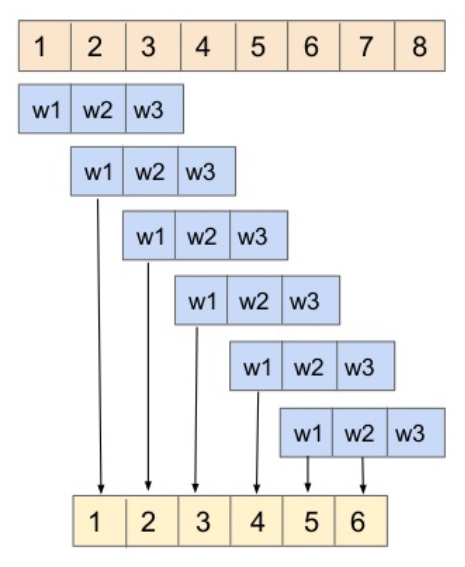
\includegraphics[width=0.3\textwidth]{1dconv_nopad}
	\caption{Convolutions in 1d \cite{catalunya_2017}}
	\label{1dconv}
\end{wrapfigure}
This architecture associates adjacent MFCC’s with each other in a hierarchical fashion. It could be hypothesised that during speech the changes in pitch/frequency occur in a consecutive fashion, with sudden changes from different parts of the spectrum unlikely, and so this information can be compressed/summarised… No padding was used, and although this means central coefficients are over represented in relation to those at the edges, it could also be hypothesised that these occur less often and, being at the edges of the frequency spectrum, are less critical to comprehension, thus features can be reduced further. As in 2d convolutions, the exact nature of the filters are left to be learned during the optimisation (back propogation?) process. 12 filters in 2 convolution layers gives 24 parameters to be learned.
The 1D convolutions output tensors of shape (V-(F-1),NF ), V is the feature vector size, NF is number of filters. To produce the correct shape for the dense layer, the tensors are flattened out to feature vectors again. In the original implementation by Sabater, he applies the ReLu activation function at this point, before applying batch normalisation and dropout. These layers are then repeated until the output neuron with a sigmoid activation function. 
%----------------------------------------------------------------------------------------
\subsection{Activation Functions}
The activation functions provide the mathematical function that emulates the nonlinear, biphasal response in the brain. For all the internal layers the ReLU function was used as this is less computationally expensive than the sigmoid where all neurons are guaranteed to fire at all times, and the use of a dropout layer removes these dying neurons to give a sparser output. 
The output activation function was a sigmoid, which is well suited for classification and ensures that all outputs from the final dense layer will be evaluated.

\begin{figure}[h]
	\centering
	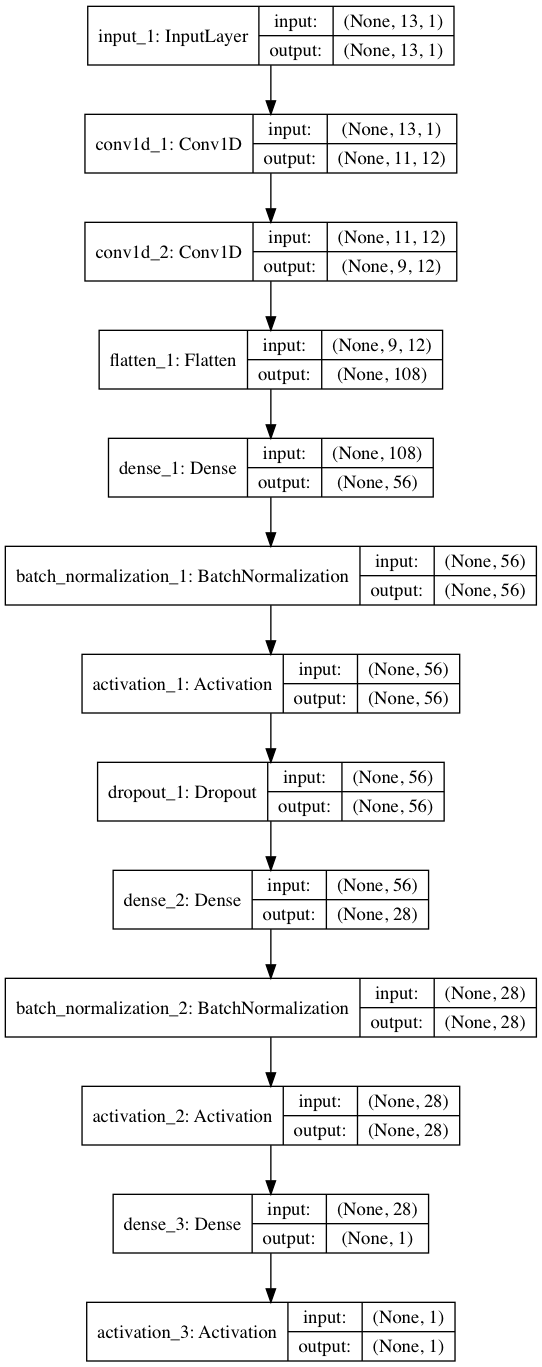
\includegraphics[height=\textheight]{model_plot_normswap}
	\caption{Model Architecture}
	\label{architecture}
\end{figure}

\subsection{Batch Normalisation}
I didn’t normalise the features directly since this relies on having the full dataset and when deployed it would not be possible to do this since we are only granted access to the dataset incrementally.
In order to learn, it is most effective when the training and test data have the same distribution. However, at each layer the outputs retain this relation only weakly due to the non-linearity of the activation functions, a process known as “internal covariance shift”, and so at each layer the new distribution must be relearnt. In addition, due to the flattening of the sigmoid function at larger values, the optimisation process slows as the gradient varies less over fixed learning rates. This can be compensated for by renormalising after every layer, but In order to normalise, the mean and variance is computed across the whole training set, but this is expensive and “not differentiable everywhere”. Instead, batchnorm stochastically computes the mean and variance over much smaller overlapping batches. This can be seen as having a regularising effect as the outputs through each layer are now dependent on what other examples were present in that batch via the mean and variation with which it is normalised rather than being processed independently. Since this process can be done several times, a single example can be related to many other examples. At test time, the learned features of the gaussian are fixed and applied to the data to give deterministic responses.
In order to compensate for this, the outputs can be normalised to a gaussian with zero mean and unit variance across each of the dimensions, output xhat. In order to ensure that the activation functions are thus not constrained to this gaussian distribution, a further transformation is made: $y = \gamma  \hat{x} + \beta$, and incorporate these new parameters into the learning process to be identified via backpropogation, hence different distributions can be inferred directly.

\subsection{Dropout}
Dropout is one method of limiting overtraining and the interdependence of neurons within layers. Nodes are defined to be active in a stochastic function as determined by a probability parameter. Hence when training, every time a sample is propagated through the network a random subset, in proportion to the probability parameter, of the neurons will not produce any output. Hence, later layers cannot depend on the presence of all inputs and reduces the tendency of neurons to co-adapt, activating in similar ways to other neurons and hence not providing additional information. In this way, a much larger set of network configurations is randomly sampled, and hence can be viewed as operating as an ensemble method for 1 hidden layer, different for more than 1.. All architectures share weights – whenever we use a hidden unit its got the same weights as it has in other architectures. Extreme form of bagging – very large number of architectures trained on just 1 sample. Sharing of weights means that every model is very strongly regularised – the weights learned from 1 architecture are stored before the architecture is sampled again. A dropout value of 0.2 was applied.

\section{Tuning}
Once the general neural network architecture was decided, there were still a range of hyperparameters to tune. In order to evaluate the effect of different optimisers, batch size and number of epochs, the hyperas package was used. This enables models with different parameters to be evaluated and the optimal parameters identified using grid search cross validation and an optimisation algorithm, Tree of Parzen Estimators (TPE) was used here. http://hyperopt.github.io/hyperopt/.
The range of parameters tested was: 
batch\_size=[32, 64, 128],
epochs=[1, 2, 3, 4, 5, 6, 7, 8, 9, 10, 50, 100],
optimizer=['SGD', 'RMSprop', 'Adagrad', 'Adadelta', 'Adam', 'Adamax', 'Nadam'],
In so doing, the best performing parameters were identified to be:
optimiser = Nadam, batch size = 32. [However, due to the random initialisation process this produced different results every time...]
\section{Training/Test Set Size}
\begin{wrapfigure}{l}{0.3\textwidth} 
	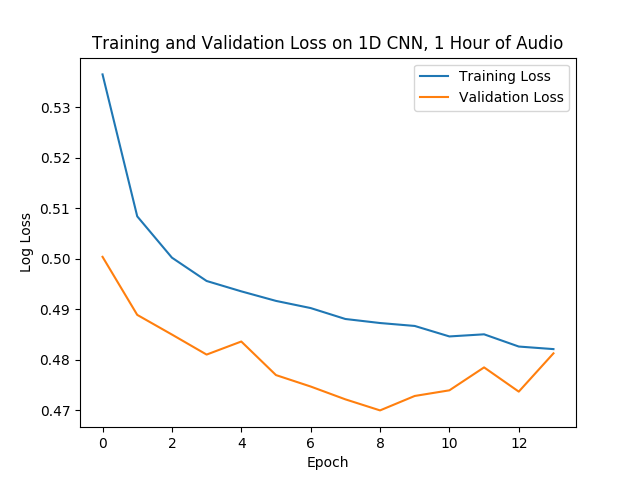
\includegraphics[width=0.3\textwidth]{train_val_loss_run2}
	\caption{Validated on a separate episode of The Walking Dead}
	\label{val_loss}
\end{wrapfigure}
In order to identify the size of training set required, the optimised learner was run on a separate validation set and the loss evaluated with epoch to see how training accuracy would improve with more data. What was thought to be a small dataset consisting of 1 hour of audio from The Walking Dead in fact was enough for the log-loss plot to indicate that the best results achievable had already been done so, and no more data would be required to replicate the results on data with a similar distribution.
Interestingly the validation loss is less than the training loss..
The validation results gave [0.81, 0.50] [accuracy, loss], which emulated closely the training results. This indicated that an hour of audio should be sufficient, but to ensure success, a full feature film was used for training.

\section{Test Time}
Prior to tuning, the model achieved respectable results Validation Loss: 0.47
Validation Accuracy: 0.76
Time:  $\sim103$ seconds

After tuning, these results were improved slightly:
Validation Loss: 0.48
Validation Accuracy: 0.81

The model was then evaluated on a full feature film, Goldstone and produced similar results:

Validation Loss: 0.49
Validation Accuracy: 0.84
Time: $\sim259$ seconds

However, there is some debate over the position of the batch normalisation layer and whether it should be placed before or after the activation [sources here], and so the tests were rerun with this swap implemented. 
In doing so, the training time and accuracy were improved significantly

Validation Loss: 0.50
Validation Accuracy: 0.93
Time: $\sim216$ seconds

suggesting better generalisation at test time.
